\chapter{Introduction}\label{}

\section{What is GEOtop}

%GEOtop has a 3D solver of Richards equation (with a Newton-Krylov method) that exchanges water with a surface (shallow water, 2D) module (explicit: probably your solver is better). The system ha also 1D solver for the energy budget in soil (well we wrote the equations in 3D but we solve just the 1D vertical). Energy is coupled to the mass transfer trough several fields that concur to determine soil heat capacity and other quantities. The energy budget include liquid-solid phase transition of liquid water into ice (and viceversa) and the deposition and metamorphism of snow (snow and can grow, and exists a mechanism for creating new layers when it grows too much). 

\begin{figure}[!h]
\begin{center}
  \begin{minipage}[c]{.80\textwidth}
    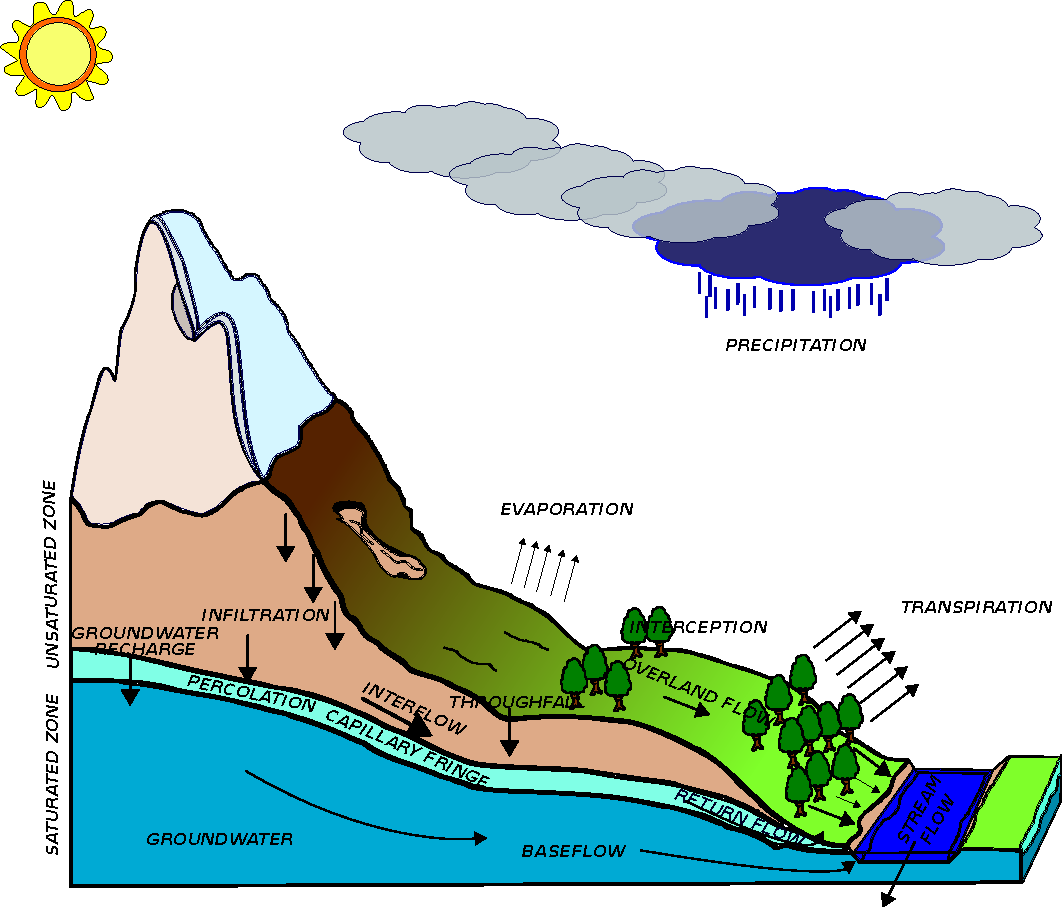
\includegraphics[width=1\textwidth]{./images/pic_general/bilancio}
    \textsl{\caption{The water cycle} \label{}}
  \end{minipage}
\end{center}
\end{figure}


Many hydrological models, commercial and research research oriented, allow to analyze the water and energy exchanges between the soil and the low atmosphere. However, often the models treat accurately only some aspects of the water cycle, i.e. the run-off or the boundary layer, and study the other parts in an approximate way.
GEOtop  \citep{Rigon06}, on the other hand, is a physically based distributed hydrological model that analyzes the complete water cycle in a catchment. The model is conceived to deal with complex topographies, as it provides each grid point of the domain with the topographical characteristics of the basin (elevation, slope, aspect, shadow, sky view factor). The soil/rock thermal and hydraulic characteristics are given in input in form of maps, together with a vertical description of the layers to account for heterogeneous stratigraphies. The vegetation and soil cover features may also be specified in form of maps.
The meteorological data, collected in one or more points in the catchment, are spatially distributed to each grid point thanks to the {\it Micromet} model \citep{liston2006meteorological}. 
Then the model calculates the energy and mass balance in the catchment through a 3D solver for Richards' equation \citep{EndrizziInvest2010} and a 1D solver for the energy equation \citep{dall2010energy}. 
The vegetation is treated according to a double layer scheme \citep{endrizzi2010observations}, that allows to separate the contribution of vegetation and of the surface on the turbulent fluxes.
The snow module, originally implemented with a monolayer scheme \citep{zanotti2004geotop}, now calculates accumulation and melting through a multilayer discretization of the snowpack \citep{endrizzi2007phd}. Recently the model has been enriched with a {\it blowing snow} module, based on \citet{pomeroy1993prairie} e \citet{essery1999distributed} contributions, that allows to account the accumulation and scour due to the wind action.
GEOtop represents a useful tool to simulate:
\begin{itemize}
\item the soil water content \citep{gebremichael2009scaling}
\item the evaporation of the soil \citep{Bertoldi2006, bertoldi2010topographical};
\item the transpiration of the vegetation \citep{endrizzi2010observations};
\item the snow in a catchment \citep{zanotti2004geotop, endrizzi2007phd, endrizzi2010observations, dallamico2011snow};
\item the surface temperature in a basin \citep{bertoldi2010topographical};
\item the temperature in the soil/rock also under freezing conditions \citep{dallamico2010phd};
\item the glacier mass balance \citep{NoldinNV2010};
\item the water table and thaw depth interactions \citep{EndrizziInvest2010};
\item and the water discharge in an outlet \citep{Rigon06}
\end{itemize}



\begin{figure}[!h]
\begin{center}
  \begin{minipage}[c]{.80\textwidth}
    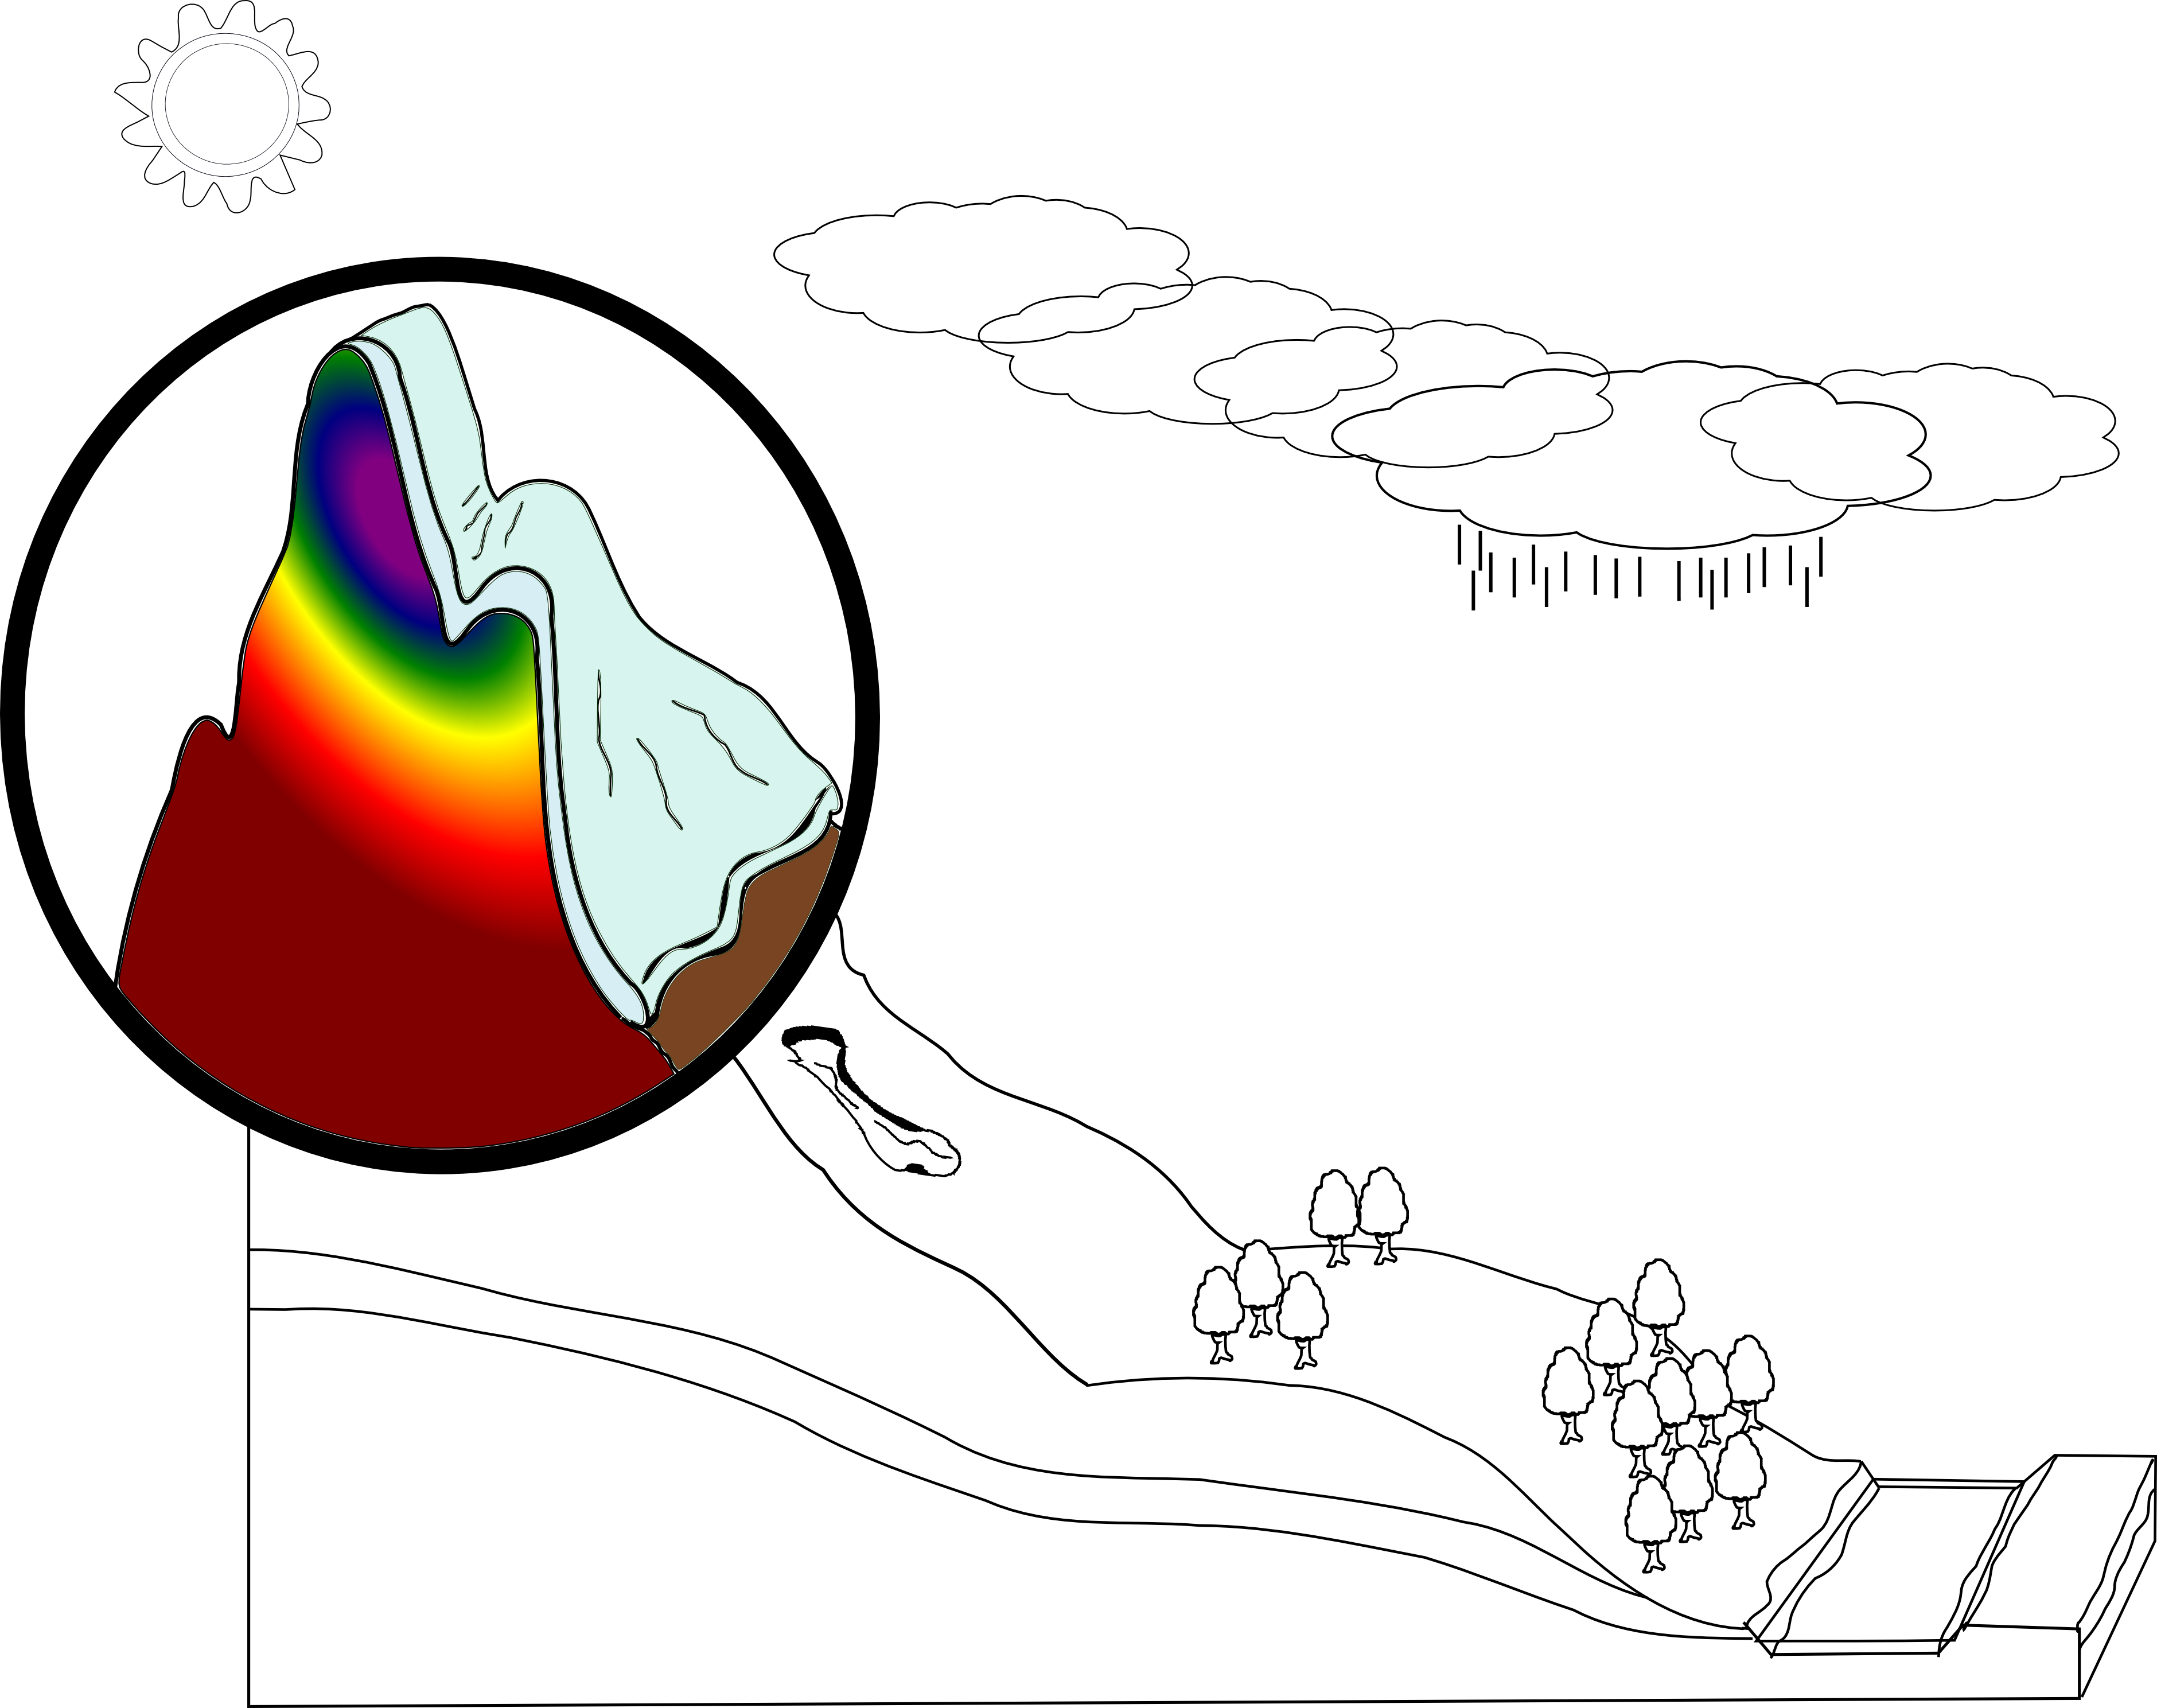
\includegraphics[width=0.7\textwidth]{./images/pic_template/criosfera_temp_grad.png}
    \textsl{\caption{Cryosphere: snow, glacier, permafrost} \label{}}
  \end{minipage}
\end{center}
\end{figure}



\begin{figure}[!h]
\begin{center}
  \begin{minipage}[c]{.80\textwidth}
    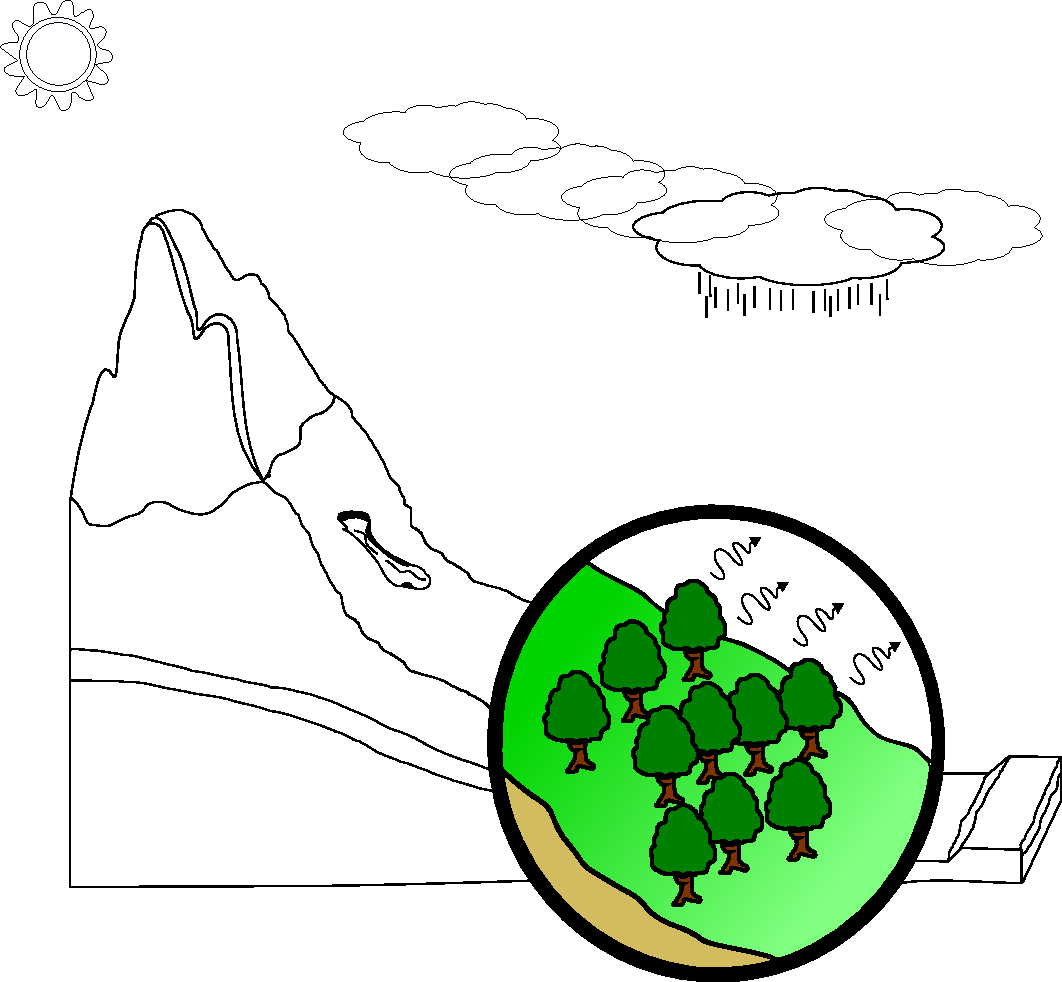
\includegraphics[width=0.7\textwidth]{./images/pic_template/vegetazione.pdf}
    \textsl{\caption{Vegetation and surface fluxes} \label{}}
  \end{minipage}
\end{center}
\end{figure}


\begin{figure}[!h]
\begin{center}
  \begin{minipage}[c]{.80\textwidth}
    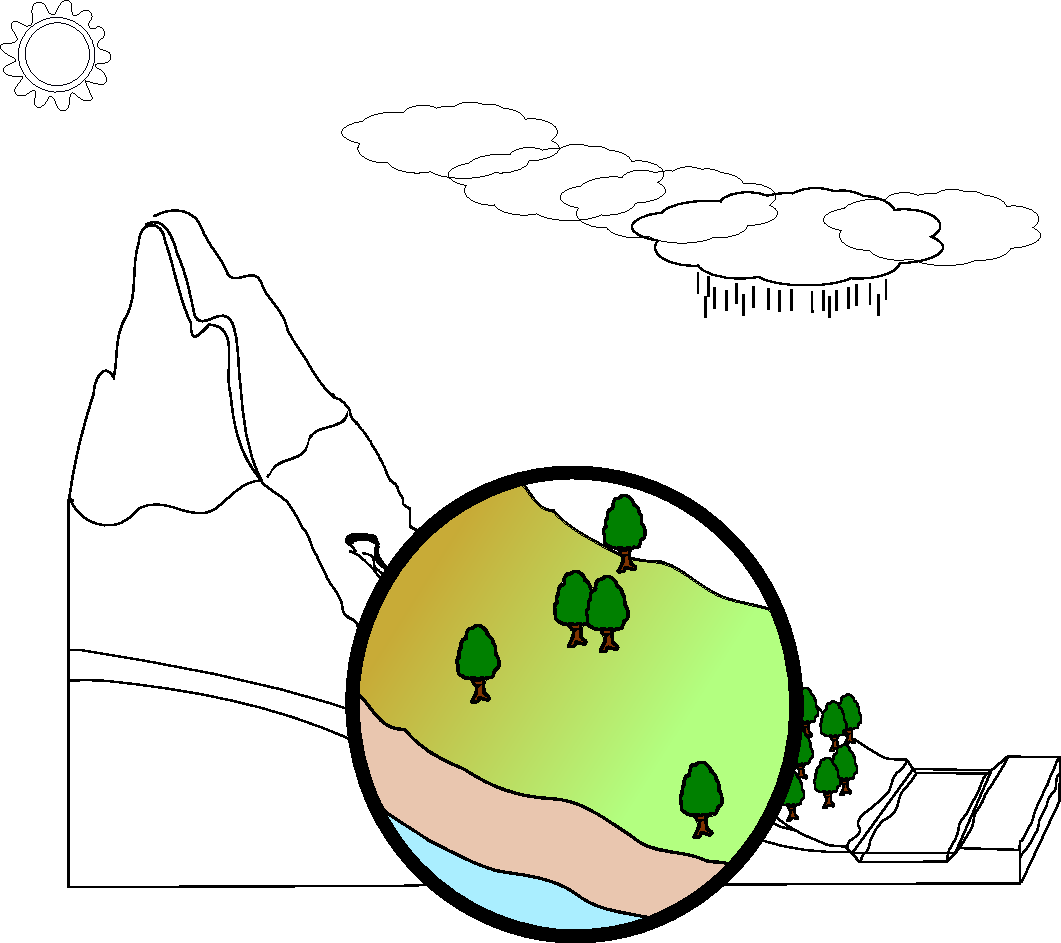
\includegraphics[width=0.7\textwidth]{./images/pic_template/suolo.pdf}
    \textsl{\caption{Soil: infiltration, water content, discharge} \label{}}
  \end{minipage}
\end{center}
\end{figure}


%\begin{figure}[!h]
%\begin{center}
%  \begin{minipage}[c]{.80\textwidth}
%    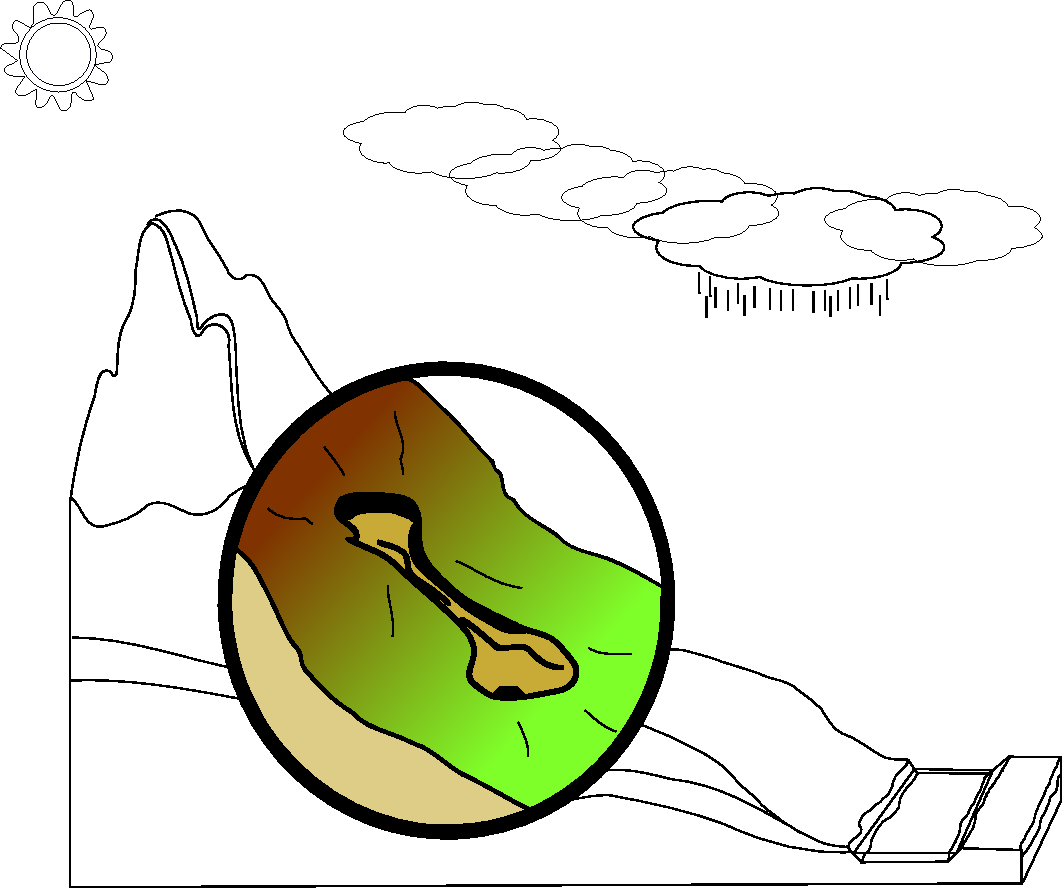
\includegraphics[width=1\textwidth]{./images/schemi/dissesti.pdf}
%    \textsl{\caption{Shallow landslides} \label{}}
%  \end{minipage}
%\end{center}
%\end{figure}

\section{History}
GEOtop concise history up to the first public release - by Riccardo Rigon

``{\it As scientists we are intrigued by the possibility of assembling our knowledge into a neat package to show that we do, after all, understand our science and its complex interrelated phenomena.}'' (W.M., Kohler, 1969). 

\subsection{GEOtop 0.5}
The first version of GEOtop (0.5) was mostly financed by the Autonomous Province of Trento through the Serraia project and by the Italian Ministry of Research and University through the Cofin 1999 project.
The very first step was due to the reading of the Entekhaby review of moddling the whole hydrological cycle [e.g. - Marani and Rigon (eds), 1997], and started with  the master thesis of Paolo Verardo and his subsequent work in 1998. Around a year was spent to implement a decent model for evapotranspiration in a complex terrain environment, according to the Penman-Monteith (PM) schematization, and all the necessary incoming radiation treatments.
 Especially the view angle and the shadowing routine were delicate to implement. The  problem of data assimilation and regionalization (at that time the only data we had were those coming from traditional hydro-meteorological stations and we do not have many of them) was face for the first time. 
Apart from the geomorphological data that we extract from DEMs (the "sine qua non" basis of all the work) we had to regionalize: air-surface temperature (varying obviously with the elevation of the terrain), net radiation (that has to be first derived from that at the atmosphere top by the evaluation of an atmospheric thickness which has to be regionalized too) and wind speed. 
In sequence it was decided decided to use: kriging  techniques and the hypothesis of adiabatic temperature profile (for air temperature); Brutsaert [1983] paper results (for atmosphere emissivity) and constant (or kriged) wind speed everywhere. 

The heat conduction into the ground was parametrized as a linear combination of a sinusoidal function as Entekhaby suggested [1997] (this has been eventually changed). That work  was also inspired by the routines  of IPW (Image Processing Workbench) [Frew, 1990]. 
Actually it was tried to get IPW working: but its pervasive scripting base (scripting is good but there is a point after which it makes the code organization unclear), the discontinued support and ignorance of IPW code internals, led  to built a new system from the scratch. 

Despite of the approximations introduced, GEOtop 0.5 model worked fairly well in estimating the net longwave and shortwave radiation in any point across a basin and at any hour of the day, and could give also reliable estimates of the potential evapotranspiration on a daily basis. However to obtain the real evapotranspiration was a different question (and, obviously, to validate it, eve a different one).  
Marco Pegoretti [1999] added to the evapotranspiration modules a rainfall-runoff model (temporary called GEOMODEL). The approach to the problem of rainfall-runoff  was strongly influenced by the work of Rodriguez-Iturbe and Valdes [1979] and Gupta et al [1980],  and I was reluctant to abandon the simplicity of a GIUH-based model in favor of a fully distributed model. 

Of the many ideas behind the theory of the GIUH there is the observation that the river basin is a complex system (an interplay of hillslopes and channels) but, at least for the forecasting of floods, just a simple model works leading to the conclusion that dynamics works in simplifying  statistically the complexity and the heterogeneity underneath.

The big problem in the GIUH approach however was (and is) the determination of the effective rainfall, i.e. the correct separation of surface runoff (interpreted as the cause of the flood surge) from subsurface flow (which must be actually treated separately and routed to the channels in a slower way), especially in dependence of storm events of diverse intensity, duration and inter-arrival time. 

A model more or less contemporary to the GIUH is the TOPMODEL by Beven and Kirkby [1979]. It is based on the paradigm that runoff production is due to saturated areas (according to Dunne and Black, 1970). Thus, once one knows which areas are saturated and describes their growing during an event, the problem of the runoff coefficient is almost solved while routing of water to an outlet can be accomplished by some simple mechanism (the Muskingum-Cunge model at least in the original papers). 
Thus, an idea could have been to merge the best of the two formulations, the GIUH concept with the TOPMODEL. However the hypothesis on which the TOPMODEL has been based, mainly the stationarity of the hillslope subsurface fluxes,  in one way simplifies the life of the modeler, but on the other is from many points of view a limitation which needs several work-around as described in  Beven et al., [2002]. In fact, when the final goal is not simply the production of a well-fitted flood wave, but for instance the estimation of local soil moisture contents, the TOPMODEL fails to be precise enough [e.g., Grayson and Wilson, 2002]. 

Furthermore, the parameters entering the model become "effective'' parameters and lose their original physical significance (for instance, the hydraulic conductivity cannot be validated by local field measurements), and need to be "calibrated" ex-post. Other limitations will be mentioned below when talking about the GEOTP 0.875 version. In any case, the TOPMODEL concept has been demonstrated to be a good tool to model floods in small-to -medium catchments, and has been considered the reference hydrological model for many of the researchers during the '90s. The TOPMODEL's ability to forecast floods derives also from its account (trivial indeed) of the topology and geometry of small- catchment flow paths: it was shown, in fact, that in small watersheds (up to at least 1000 square kilometers), hillslope residence time dominates the characteristic time of flood formation and that topology and geometry of river basins are sufficient with very minimalist dynamics to explain the shape of floods [Rinaldo et al, 1991; Rigon et al, 1996, Rinaldo et al., 1995, D'Odorico, 1996; D'Odorico and Rigon, 2003]. 
Thus, it was decided  to build completely new subsurface and surface models, still driven by gravity (i.e. by slope as the TOPMODEL and not by the total hydraulic head) but, as a first approximation to the final wishes, introducing the buffer to cope with infiltration into the vadose zone.  Subsurface flow was produced only by the saturated layer (including the capillary fringe), if present, and lateral surface runoff was routed as a kinematic wave (and through Manning/Gauckler-Strikler equation for velocities). 

In doing this, it was searched  a better characterization of flow paths, with reference to the bedrock, instead of to the surface topography [see McDonnell et al., 1996]: this could be done by measuring soil depth or interpolating it for instance as in [Heimsath et al, 1997 or Roering et al, 1999; please see the overlooked  Bertoldi et al, 2006 for the details]. 

In this separation of surface and subsurface fluxes, GEOtop 0.5 was similar to the grid bases THALES [Grayson et al., 1994a,1994b] or the more recent NEWTHALES. At first, the version of GEOtop by Verardo-Pregoretti-Rigon (GEOTOP 0.5) could work without an explicit channel routing assigning a locally variable roughness and hydraulic radius; usually, however, channels were determined by accurate topographic analysis and explicitly treated. Channels routing was performed by a GIUH theory as in Rinaldo et al [1995], where channel celerity and hydrodynamic dispersion were  considered spatially uniform and constant in time. 

Instead of the effective rainfall, the spatially an temporally distributed input to channels was produced by GEOtop, i.e. the GEOMODEL produced patterns of spatially distributed soil moisture, and these patterns were used to reduce the potential evapotranspiration to its real counterpart as described in Bertoldi et al., [2002]. 

\subsection{GEOtop 0.75}
(mostly financed by COFIN 2001, THARMIT Eu Project, CUDAM - CofinLab 2001, ASI 54/2000)

The use of PM  equation for evapotranspiration was indeed unsatisfactory from many points of view. For instance, it depends on air temperature that was derived from interpolation, and it was envisioned that  the parametrization of fluxes into the ground, sensitive both to the ground cover and to the water content, could be modeled directly, haven as a  result that many of the variables and parameters that were known to be correlated were actually treated separately.
 
Thus, with the Master thesis of Giacomo Bertoldi[2000] wit was decided throw away the PM equation (actually we kept it for comparison), and to solve directly the energy balance in any point of the basin. This was the birth of GEOTOP 0.75 which is thoroughly documented in Bertoldi et al[2002a,b] and Rigon et al [2002]. It was actually a SVAT model plus an rainfall-runoff model coupled together. GEOtop needed several parameters to be run, however the modeling could have been considered parsimonious, if all the prognostic capabilities were to be considered.   The user could switch-off the SVAT part and have a parametrically parsimonious rainfall-runoff model, or vice-versa she can switch-off the rainfall-runoff model and have a reasonably simple SVAT model. 
Large efforts were  done in cleaning the old code and improving the input-outputs. Credits must be given to the work of Liang et al. [1994] with their work on VIC (which is however parametrized to work at much larger scales) and on Wigmosta et al. [1994] whose model is very similar to the version 0.75 of GEOtop (but was mostly a case of evolutionary convergence since the comparison came after the GEOtop implementation). 
From the beginning,  the model was used  to forecast the whole hydrological cycle, even if a reasonable snow modeling still had to arrive. We were looking also to other topics. 
 Eco-hydrology was, in fact, a research thread whose seeds where already in Rodriguez-Iturbe's mind when I was working with him at the Texas A\&M University (1994-1996) and of which I was concerned from the beginning of the project. 

Ecohydrology [Rodriguez-Iturbe, 2000] has roots in the work of Eagleson [1978, 2003], Phili, Brutsaert, Hillel [1990],s and others and is one of the hot issues in these hydrological decades [Rodriguez-Iturbe, 2000]. 

For validation of the modules, a key role in this had Tom Over who, besides giving a lot of suggestions making the concepts behind the model clear, suggested to use the South Great Planes 97 experiment data set, thing that we promptly did as it appears in the first journal paper about the model Rigon et al., 2006). 

Based partially on GEOtop 0.75 (and on the subsequent GEOtop 0.875) came all the work by Reza Entezarolmahdi who tried first to create an automatic calibration system for the model. This actually used MOSC-EM [CITATIONS] which, however was never really integrated in the model.  The work of Reza was really interesting for many point of view, but probably a little advanced with respect to times and finished to a dead-end from which we hope to resume it sometimes in the very next future. 

\subsection{GEOtop 0.875}
(mostly financed by TIDE EU Project, CUDAM Cofinlab COFIN 2001, THARMIT EU project)

This version finally contained a snow accumulation and melt model (derived by the Utah Energy Balance -UEB- by Tarboton and Luce, [1992]) implemented by Fabrizio Zanotti [2003] with the help of Giacomo Bertoldi .  It also included a post-processor, the S-FACTOR , which performed a landslide and debris-flow triggering implemented by Christian Tiso [2003] (eventually evaluated into GEOtop-SF by Silvia Simoni).  Both the implementations were the outcome of two M.S. thesis.  Snow-melting and soil freezing are essential components in the hydrological cycle of mountain catchments and cannot not be overlooked. Landslide and debris-flow triggering are also an issue with particular relevance in mountains areas, such that floods in mountain areas are usually the combined effect of large liquid and solid discharges whose effects cannot be separated: GEOtop with this version started to a tool for studying these phenomena. 

However, with the version 0.875, we wanted to attack the problem of a sound hillslope-hydrology modeling. 

So far, our understanding of mountain catchments in fact was based on hillslope hydrology, as reviewed for instance in Wipkey and Kirkby [1978], and  the "perceptual" hillslope model that we had at that time derived from the assumption that it was possible to neglect the transients in the water fluxes [in the sense clarified in Iverson, 2000]; that topographic gradients dominate the hydrologic response; that hydraulic conductivity strongly decreases with depth in the soil and, not independently, that runoff occurs mostly owing to saturation excess. 
This last assumption in turn was  based upon the results of a long series of experiments from the late seventies on by American geomormologists (Dunne, Black, Dietrich, Montgomery, Torres), and was supported by many others (among these: Moore, Grayson, Sivapalan, Wood). 
These experiments and subsequent research activities changed the belief spread by Horton that runoff was mostly due to the infiltration excess mechanism. Developing hydrological models based on saturation excess ideas (which involved further simplification) originated a series of rainfall-runoff models among which the already cited TOPMODEL [Beven and Kirkby,1979; Sivapalan et al, 1991; Franchini et al, 1996] is the most successful product. 
 
There are many aspects that could be improved with respect with that model. For instance,  in characterizing  the subsurface flow field more in terms of total head, even if in simplified form as in Iverson [2000], than in terms of the topographic gradient, as a first step toward the integration of the three dimensional Richards equation. These  steps were implemented by the master thesis of Davide Tamanini [2003] that made GEOtop able to simulate transient subsurface flow, and both saturation excess and infiltration excess runoff.  A first parameterization of the soil water retention curves was also implemented in the model. It is this code that was used in the first journal papers on GEOtop (Zanotti et al., 2004, Rigon et al., 2006, Bertoldi et al., 2006). Upon this code was based the work by Silvia Simoni, helped by Fabrizio Zanotti which produced the GEOtop-SF postprocessor that was able to estimate statistics of the stability of a hillslope. This work, in turn, produced Simoni Ph.D. thesis  and Simoni et al., [2008]. 

In GEOtop 0.875 the integration of Richards equation followed a custom numerical scheme that was exceedingly complicate and non standard. Moreover, the integration scheme was not fully 3D, but could have been defined 2D + 1D, where "2D" stands for the lateral flow, obtained by using the Darcy Buckingham law, and 1D was the resolution of a one dimensional Richards equation. Despite these limitations, we could obtain reasonable reproduction of soil moisture distributions,  good discharges at the outlet of basins, excellent reproduction of summer soil temperatures, and what we considered a good reproduction of turbulent heat and evapotranspiration exchanges. 


\subsection{GEOtop 0.9375}
 and subsequent version till the first public release
(mainly financed by Projects with Servizio geologico PAT, progetto MORFEO by ASI, and EU IRASMOS and  AQUATERRA projects)

The new development started with in mind that we had sooner or later to switch to a version of GEOtop with a full 3D integration of Richards equation. 

However, the first new improvement of GEOtop was in the direction to include a multiple layer  modeling of snow and a first core of the freezing soil subroutines.  This was mainly accomplished during the Ph.S thesis of Stefano Endrizzi [2007], and greatly improved in his subsequent work at Saskatoon, working with Phil Marsh and Bill Quinton, and recently at Zurich University collaborating with  Stephan Gruber. 

Why complicating even more an already complex model? Moreover, why getting a new snow model, if the Utah energy balance seemed to work fine, as written in Zanotti et al., 2004?
The rational behind this choice was essentially that the snow water equivalent was not enough for comparing snow measurement in the field with model outcomes. Clearly snow water equivalent (SWE) was enough just for those willing to cope with total water volume generated after snow melting, but not sufficient for studying and understanding the processes behind snowpack evolution and ablation. Nor even for having a reasonable estimate of soil temperature under the snow, and other interesting prognostics, like snow density. 

However, Stefano's efforts were not limited to snow. He worked hard, for getting a consistent integrator of Richards equation, that he based on a Newton Krilov-method (Kelley, 2003).  Besides he decided to change the surface water flow  equation and numerics, by using the shallow water equation integrated with a robust but explicit method.  This resulted in a very stable and reliable code that constitutes the core of the first public version of GEOtop. In fact Stefano decided to move from the the fraction of geometric series of  $\sum_i (1/2)^i$ to the integer 1.

The collaboration of Stefano and Matteo Dall'Amico produced also a consistent integrator of the freezing soil moisture, after that Matteo, in his Ph.D thesis disentangled, at least for ourselves,  a lot of thermodynamics (and together, we introduced a simple, and "normal" thermodynamic notation). This work has been documented in Dall'Amico et al., 2010 LINK, and produced a paper for The Cryosphere LINK. 

\subsection{Stefano Endrizzi's work}

Up to version 0.875 version GEOtop was pretty much a home made effort, mainly pursued by Master and Ph.D students of Trento University. However, since then, either because the Ph.D students became doctors and spread around, and because other discovered the potential our work, GEOtop started to became really internationally used. Han Xunjun in China used GEOtop in his data assimilation system implementing an ensemble Kalman filter (in Python). The Lausanne group under the direction of Marc Parlange, within the collaboration of Silvia Simoni, and the direct coding efforts of Thomas Egger implemented a real time version of the model that is giving its results everyday (http://lsir-hydrosys01.epfl.ch:22006/). John Albertson and his group implemented an erosion module to be coupled with GEOtop. In Trento, a version of GEOtop, called GEOtop-EO implemented a prototype of  infrastructure that includes besides the modeling core, a geographical database, with a raster service (built upon RAMADDA -LINK) and a visualization system based on JGrass. This was done for the project MORFEO (LINK).  At Bolzano, in EURAC, Giacomo Bertoldi and Stefano Dallachiesa, endowed GEOtop with an external (so far) vegetation dynamical model (itself came from previous work by Albertson and Montaldo). Last, but not least, Mountain-eering made of GEOtop the center of its business plan, and supported the completion of the freezing soil module, and is going to develop a new NetCDF input/output system, and the creation of some data assimilation of snow measures. 

Credits to work of the group of Lousanne should be given to have also included in GEOtop the METEO/IO environment which was the way to link the model to a real-time acquisition system.  Stefano Endrizzi himself, when at Saskatoon, discovered the work of Liston and Elder [2006] with MICROMET, and included it in the GEOtop distribution with the permission of the Authors. 

Also other player came  to the game. Arpa Val D'Aosta decided to make of GEOtop the principal tool for doing analysis on snow and permafrost, and it is going to support its improvement and usability. The Karlshrue Institute of Technology in Garmisch-Partenkirchen (and particularly Prof. Harald Kunstmann, and coworkers) adopted for simulation for one of their TERENO experiment (LINK).  

This, just to mention partial developments, not all of them yet flowed into the main version of the model. All of these efforts, in fact, could not being really unified in a single product. 

\subsection{GEOtop in Zurich}


\subsection{Future perspectives}
So

So the questions for the future are: 

how can we manage the future of this international crew, letting any single her freedom ?
and making the whole community grow cooperatively ?
how giving anyone the proper credits which are necessary to go ahead ?
how maintain while moving on relevant pieces of software still available avoiding to wipe them out (as it happens for the PM coed, and more recently, with the former runoff-modules. to do a couple of examples ?

I gave already some possible direction (see for instance LINK) that derives from the issue raised by the work of Stefano Endrizzi and Hydrologis, and in an effort to unify all of my previous work lines.

However, this is not an aster I want to do by myself. The community around GEOtop must give its opinion. Because the only perfect model is the evolving one, since many contenders appear, our knowledge grows, and all of us work hard. 

Relevant Literature 
